\documentclass[colorised, sobre]{template} % Options : devie, sobre, colorised

%*  liste des auteurs, pour la page de garde
\def\listAuteurs
    {\gdbdg } % auteurs, avec \auteur{prénom}{nom}

%* liste des encadrants, utilisé dans la page de garde
\def\listEncadrants
    {\auteur{Prenom }{nom Encadrant}} % Encadrants, avec \auteur{prénom}{nom} 

%* Défini le partie avec les auteurs et encadrants de la page de garde, utilisié par \miniTitlePage et \titlePage
\def\enteteAuteurs
    {\auteurs
        {\listAuteurs} % liste des auteurs
        {\listEncadrants} % Liste des encadrants
        []  % 1 si encadrants, 0 sinon (def 0)
        [0]  % 1 si plusieurs auteurs, 0 sinon (def 0)
        [1]} % 1 si full page, 0 si mini page, (def 0) 

%* header
\header
    [serpico.png]
    {Calculs de résultats} % Titre du milieu
    {de Bigault de Granrut} % nom (l1 droite)
    {Guillaume} % prénom (l2 droite)

%* Raccourcis pour ce document
\def\ms{micro service}
\def\ser{Serpico}
\def\usr{user}
\def\te{team}
\def\st{stage}
\def\ph{phase}
\def\we{weighted}
\def\equ{equal}
\def\lb{\mbox{lb}}
\def\ub{\mbox{ub}}
\def\tp{tiers utilisateurs}
\def\weight{\mbox{weight}}
\def\result{\mbox{result}}
\def\stdDev{\mbox{stdDev}}
\def\avRe{\mbox{averageResult}}
\def\avReRe{\mbox{averageRelativeResult}}
\def\avSd{\mbox{averageStdDev}}
\def\msd{\mbox{maxStdDev}}
\def\iner{\mbox{inertia}}
\def\miner{\mbox{maxInertia}}
\def\aR{\mbox{averageResult}}
\def\arr{\mbox{averageRelativeResult}}
\def\asd{\mbox{averageStdDev}}
\def\arat{\mbox{averageRatio}}
\def\crit{\mbox{crit}}
\newcommand{\grade}[2]{\mbox{grade}[#1 \rightarrow #2]}

\begin{document}

%* Page de garde
%\miniTitlePage
\titlePage
    {serpico.png} % image de garde
    {\white{f}} % Filière
    {Notice du micro service de notation} % Main title
    {\white{s}} % Subtitle
    {\enteteAuteurs} %(que pour grande page de garde)
    %[0] % 1 si sommaire, 0 sinon (def 1)
    %[0] % 1 si liste des figures, 0 sinon (def 0)
    %[0] % 1 si liste des tableaux , 0 sinon (def 0)

%TODO Le document 
%TODO détailler mise en prod et utilisation au sein du reste du code 
\section*{Introduction}
    Ce \ms{} permet de calculer tous les résultats nécessaires au fonctionnement de la solution proposée par \ser. Ce service, totalement indépendant du reste de la solution, prends en entrée un json avec les données nécessaires, et renvoie en sortie un autre json contenant les résultats calculés. 
    Ce service permet la jockerisation.
    Ce service est développé en python.

\section{Les résulats calculés}
    Cette appli calcule des résultats pour des critères, des phases (stage), et des activités. 
    Il y a deux types de résultats : 
    \begin{itemize}
        \item[\BB] Les résultats individuels : ce sont les résultats réalisés par une entité, que ce soit un \usr, une \te, ou même une \ph. Ils se décompose en deux types de valeurs : 
        \begin{itemize}
            \item Les résultats \we : les résultats pondérés par le poids des notés et des notants, selon utilisation dans les formules.
            \item Les résultats \equ : les résultats non pondérés, ce qui équivaut à utiliser une pondération de 1.
        \end{itemize}
        Dans un souci de simplification, les formules seront détaillées une seule fois, avec la pondération.
        \item[\BB] Les résultats globaux : c'est des moyennes sur les différents critères, ainsi que quelque autres paramètres calculés. Ils se décomposent en 4 cas (plus en compant les valeurs avec un maximum théorique) :
        \begin{itemize}
            \item Les valeurs sur les \usr : moyennes calculées sur les \usr, et non les \te. Elles se décomposent également en \we{} et \equ.
            \item Les valeurs sur les \te : moyennes calculées sur les \te, et pas les \usr. Elles se décomposent également en \we{} et \equ.
        \end{itemize}  
        Dans un souci de simplification et de lisibilité, les formules seront détaillées que dans un seul cas (pondéré). Il suffira de remplacer par les populations correspondantes.
    \end{itemize}
    \subsection{Traitement de la jockerisation}
    Le moyen le plus simple de  traiter la jockerisation est simplement de ne rien renseigner quand une note est manquante, l'application bouclera sur les notes renseignées, et fera les calculs de pondérations en conséquence. Le seul défaut est de devoir calculer la somme des poids pour chaque entité, ce qui est peu couteux. Pour le calcul des résultats globaux, on utilise les moyennes comme avant, car changer les formules aurait peu de sens, et apporterait uniquement de la complexité pour rien, et ne causerait que des problèmes.
    \subsection{Pour un critère}
        Cette partie est la plus importante. Elle process l'ensemble des notes. Voici les résultats calculés : 
        \subsubsection{Les résultats individuels}
            On note : 
            \begin{itemize}
                \item[\BB] grade[grader $\rightarrow$ grader] : la note donnée par grader à graded
                \item[\BB] graders(u) : perosnnes évaluant u (si u apparient à une \te, prends en compte la note attribuée à sa \te)
                \item[\BB] graded(u) : les personnes évaluées par u (peut varier à cause de la jockerisation)
                \item[\BB] graders : ensemble des notants du critère (décrit soit l'ensembe des \usr, soit des \te{} contenant au moins un \usr{} notant).
                \item[\BB] graded : ensemble des entités évaluées pour ce critère.
                \item[\BB] result(u) : le résultat de u
                \item[\BB] weight(u) : le poids de u
                \item[\BB] relativeResult(u) : le résultat relatif de u
                \item[\BB] stdDev(u) : l'écart type de u
                \item[\BB] team : membres de la team de 
            \end{itemize}  
            Les résultats individuels sont :   
            \begin{itemize}
                \item Result : simplement la moyenne de résultat pour un critère, résultat concernant les notés, soit les actifs et les passifs.
                \begin{eq}
                    \result(u) = \sum_{g \in \mbox{graders}(u)} \dfrac{ \grade{g}{u} \times \weight(g)}{\sum_{g \in \mbox{graders}(u)} \weight(g)}\\
                \end{eq}
                \item RelativeResult : formule appliquée à la moyenne de résultat, qui donne une idée de celle-ci, sans avoir les bornes de la note.
                \begin{eq}
                    \mbox{relativeResult}(u) = \dfrac{ \result(u) - \lb}{\ub - \lb}\\
                \end{eq}
                \item stdDev : concerne les notants (les \tp et les actifs). Cet écart type est réalisé sur les notes \emph{données} et non pas reçues. Il décrit à quel point l'utilisateur est d'accord avec les autres notants.
                Il vaut : 
                \begin{itemize}
                    \item pour les \usr
                    \begin{eq}
                        \mbox{stdDev}(u) = \sqrt{\sum_{g \in \mbox{graded}(u)} \dfrac{ (\grade{u}{g} - \result(g))^2 \times \weight(g)}{ \sum_{g \in \mbox{graded}(u)} \weight(g)} }\\ 
                    \end{eq}
                    \item pour les \te
                    \begin{eq}
                        \mbox{stdDev}(\mbox{team}) = \sum_{g \in \mbox{team}} \dfrac{\mbox{stdDev}(g) \times \weight(g)}{\sum_{g \in \mbox{team}} \weight(g)} \\ 
                    \end{eq}
                \end{itemize}
                
                \item devRatio : un écart type ne parlant pas forcément, \ser{} propose un ratio entre l'acart type et un maximum théorique d'écart type.
                Il vaut : 
                \begin{eq}
                    \mbox{devRatio}(u) = \dfrac{\mbox{stdDev}(u)}{\mbox{maxStdDev}}
                \end{eq}
                maxStdDev est l'écart type maximum théorique possible. Son calcul est détaillé plus bas. Il prend une valeur différente selon qu'on traite un \usr{} ou une \te. 
            \end{itemize}
        \subsubsection{Les résultats globaux (moyenne sur le critère)}
            Les résultats globaux sont (pour rappel, en 4 fois, selon pondération et \te{} ou \usr) : 
            \begin{itemize}
                \item averageResult : moyenne des résultats sur le critère. Cette valeur n'est calculée que si les bornes de notation sont les mêmes pour tous les critères (n'a pas de sens sinon, est set à \texttt{null}).
                \begin{eq}
                    \avRe = \sum_{g \in \mbox{graded}} \dfrac{\result(g) * \weight(g)}{\sum_{g \in \mbox{graded}(u)}\weight(g)}\\
                \end{eq}
                \item averageRelativeResult : même principe que pour le résultat relatif individuel.
                \begin{eq}
                    \avReRe = \dfrac{\avRe - \lb}{\ub - \lb}\\
                \end{eq}
                \item averageStdDev : moyenne des écarts types.
                \begin{eq}
                    \avSd = \sum_{g \in \mbox{grader}} \dfrac{\stdDev(g) \times \weight(g)}{\sum_{g \in \mbox{grader}} \weight(g)}\\
                \end{eq}
                \item maxStdDev : maximum théorique des écarts types.
                \begin{eq}
                    \msd = \sum_{g \in \mbox{graded}} \dfrac{\max(\ub - \result(g), \result(g) - \lb)}{\sum_{g \in \mbox{graded}} \weight(g)}\\
                \end{eq}
                \item inertia : inertie des écarts type : 
                \begin{eq}
                    \iner =  \sum_{g \in \mbox{grader}} \dfrac{\stdDev(g)^2 \times \weight(g)}{\sum_{g \in \mbox{grader}} \weight(g)}\\
                \end{eq}
                \item maxInertia : carré de maxStdDev
                \begin{eq}
                    \miner = \msd^2\\
                \end{eq}
                \item les devRatio : le ratio de l'Inertie
                \begin{eq}
                    \mbox{devRatio} = \dfrac \iner \miner \\
                \end{eq}
            \end{itemize}


    \subsection{Pour une phase ou une activité}
    \ser{} propose de calculer un certains nombre de moyennes sur les phases et activités. Comme le principe est le même pour une phase ou une activité, nous ne détaillerons les calculs qu'une seule fois, il faut prendre la population parmis les critères ou les phases, selon qu'on fasse les moyenes pour un phase ou une activité. Encore une fois, ces résultats sont calculés dans le cas pondéré et \equ, et \usr{} ou \te{} pour les valeurs globales. 
    
    On utilise les notations suivantes, dans le cas où elles sont définies : 
    \begin{itemize}
        \item result[u,crit] : le résultat (moyenne sur un critère ou phase) de u sur crit (un critère ou une phase).
        \item relativeResult[u,crit] : le résultat relatif de u sur crit.
        \item stdDev[u,crit] : l'écart type (moyenne sur un critère ou phase) de u sur crit (un critère ou une phase).
        \item devRatio[u,crit] : le ratio de déviation de u sur crit.
        \item weight(crit) : le poids du critère, nécessairement défini.
        \item Crit : soit l'ensemble des critères, ou des phases, selon l'élément traité.
    \end{itemize}
    \subsubsection{Les résulats individuels}
        \begin{itemize}
            \item les moyennes de résultats (on parle aussi de résultat absolu dans le code existant de \ser).
            \begin{eq}
                \aR(u) = \sum_{c \in \crit} \dfrac{ \result(u) [u,c]}{\sum_{c \in \crit} \weight(c)} \\
            \end{eq}
            \item les moyennes de résultats relatifs 
            \begin{eq}
                \arr(u) = \sum_{c \in \crit} \dfrac{ \mbox{relativeResult} [u,c]}{\sum_{c \in \crit} \weight(c)}
            \end{eq}
            \item l'écart type moyen 
            \begin{eq}
                \asd = \sum_{c \in \crit} \dfrac{ \stdDev [u,c]}{\sum_{c \in \crit} \weight(c)}
            \end{eq}
            \item le ratio de déviation moyen : 
            \begin{eq}
                \arat = \sum_{c \in \crit} \dfrac{ \mbox{devRatio} [u,c]}{\sum_{c \in \crit} \weight(c)}
            \end{eq}
        \end{itemize}
    \subsubsection{Les résultats globaux} 
        On fait la moyenne de la même manière, sur tous les paramètres globaux calculés précédamment.
        %! todo si le chef demande, sinon non
        \textcolor{red}{Je n'ai pas détaillé les calculs, car c'est vraiment la même chose qu'au dessus. Si tu veux, je le fais, et sinon çà sera laissé au lecteur}.
\section{Les paramètres en entrée}
    Ce micro service prend en paramètre un json qui contient toutes les informations nécessaires pour calculer tous les résultats détaillés précédamment. Voici ci dessous les paramètres nécessaires : 
    \subsection{Pour les critères}
        \begin{lstlisting}
{
    "userWeights": {
        "id_user": value,
    },
    "teams":{
        "id_team":[
            "id_participant",
        ]
    }
    "teamWeight":{
        "id_team": value, 
    }
    // Not yet implemented
    "legitimity":{
            "id_graded":{
                "grader":value,
            }
        }

    "criterias": {
        "criteria_id": {
            "lowerbound": value,
            "upperbound": value,
            "user_grades": {
                "grader_id": {
                    "graded_id": value // note du graded, donnee par le grader
                    "graded_id2" : value
                }
            }
            "team_grades"{
                "grader_id": {
                    "team_id": value // note de la team, donnee par le grader (un user)
                    "team_id2" : value
                }
            }
        }
  }
}
        \end{lstlisting}
    \textcolor{red}{est ce que c'est assez clair, ou est ce que je dois détailler plus ?}
    \newpage
    \subsection{Poue les phases et activités}
        \begin{lstlisting}
{
    "globalData":{
        "weight" : 
        "averageUsersWeightedResult" : value,
        "averageUserslEqualResult." : value,
        "averageTeamWeightedResult" : value,
        "averageTeamEqualResult" : value,
        //RelativeResult
        "averageUsersWeightedRelativeResult" : value,
        "averageUserslEqualRelativeResult" : value,
        "averageTeamWeightedRelativeResult" : value, 
        "averageTeamEqualRelativeResult" : value,
        //StdDev
        "averageUsersWeightedStdDev" : value,
        "averageUsersEqualStdDev" : value,
        "averageTeamWeightedStdDev" : value,
        "averageTeamEqualStdDev" : value,
        //MaxStdDev
        "maxUsersWeightedStdDev" : value,
        "maxUsersEqualStdDev" : value,
        "maxTeamWeightedStdDev" : value,
        "maxTeamEqualStdDev" : value,
        //Inertie 
        "usersWeightedInertia" : value,
        "usersEqualInertia" : value,
        "teamWeightedInertia" : value,
        "teamEqualInertia" : value,
        //MaxInertie
        "maxUsersWeightedInertia" : value,
        "maxUsersEqualInertia" : value,
        "maxTeamWeightedInertia" : value,
        "maxTeamEqualInertia" : value,
        //Ratio
        "usersWeightedRatio" : value,
        "usersEqualRatio" : value,
        "teamWeightedRatio": value,
        "teamEqualRatio" : value,

        "user" :{
            "id_participant":{
                "weightedResult": value,
                "equalResult":value,
                "weightedRelativeResult":value,
                "equalRelativeResult":value,
                "weightedStdDev":value,
                "equalStdDev":value,
                "weightedRatioStdDev": value,
                "equalRatioStdDev": value
            }
        }
        "teams":{
            "id_participant":{
                "weightedResult": value,
                "equalResult": value,
                "weightedRelativeResult": value,
                "equalRelativeResult": value,
                "weightedStdDev": value,
                "equalStdDev": value,
                "weightedRatioStdDev": value,
                "equalRatioStdDev":value
            }
        }
    } 
}                        
        \end{lstlisting}
    \textcolor{red}{est ce que c'est assez clair, ou est ce que je dois détailler plus?}

\section{Les données en sortie}
    Les données en sortie auront toujours la même structure, que ce soit pour des calculs sur un critère, une phase, ou une activité. Cà permet notamment de faire une seule fonction de traitement dans l'appli principale.
    \begin{lstlisting}
{
    "id": {

        "averageUsersWeightedResult" : ,
        "averageUserslEqualResult." : ,
        "averageTeamWeighteResult" : ,
        "averageTeamEqualResult" : ,
        //RelativeResult
        "averageUsersWeightedRelativeResult" :,
        "averageUserslEqualRelativeResult" : ,
        "averageTeamWeighteRelativeResult" :, 
        "averageTeamEqualRelativeResult" :,
        //StdDev
        "averageUsersWeightedStdDev" :,
        "averageUsersEqualStdDev" : ,
        "averageTeamWeightedStdDev" : ,
        "averageTeamEqualStdDev" : ,
        //MaxStdDev
        "maxUsersWeightedStdDev" : ,
        "maxUsersEqualStdDev" : ,
        "maxTeamWeightedStdDev" : ,
        "maxTeamEqualStdDev" : ,
        //Inertie 
        "usersWeightedInertia" : ,
        "usersEqualInertia" : ,
        "teamWeightedInertia" : ,
        "teamEqualInertia" : ,
        //MaxInertie
        "maxUsersWeightedInertia" : ,
        "maxUsersEqualInertia" : ,
        "maxTeamWeightedInertia" : ,
        "maxTeamEqualInertia" : ,
        //Ratio
        "usersWeightedRatio" : ,
        "usersEqualRatio" : ,
        "teamWeightedRatio": ,
        "teamEqualRatio" : ,

        "user" :{
            "id_participant":{
                "weightedResult":,
                "equalResult":,
                "weightedRelativeResult":,
                "equalRelativeResult":,
                "weightedStdDev":,
                "equalStdDev":,
                "weightedRatioStdDev":,
                "equalRatioStdDev":
            }
        }

        "team" :{
            "id_participant":{
                "weightedResult":,
                "equalResult":,
                "weightedRelativeResult":,
                "equalRelativeResult":,
                "weightedStdDev":,
                "equalStdDev":,
                "weightedRatioStdDev":,
                "equalRatioStdDev":
            }
        }
    }
}
    \end{lstlisting}
    Remarque sur \texttt{"id"}. Cette valeur n'a de sens que pour les critères, car ce framework peut en traiter plusieurs en même temps. Dans le cas des stage et des activity, cette valeur vaut \texttt{"step"}. (Ne pas la changer sans mettre à jour l'appli principale).
    
    Le choix est fait pour l'instant de ne pas regrouper les \te{} et \usr, la principale raison qui a motivé ce choix est la gestion des clés. En effet, un \usr{} et une \te{} peuvent avoir la même clé, en les séparants ainsi, on peut les renseigner avec leur vraie clé, ce qui simplifiera l'utilisation du micro service par le reste de l'appli \ser.
\section{architecture de l'appli}
    On propose une solution orientée objet, et non pas un calcul matriciel, pour plusieurs raisons.
    \begin{itemize}
        \item Une telle matrice est creuse, et c'est pire avec la jockerisation, ce qui implique de la perte en mémoire, et en performance. Surtout, çà perd en lisibilité pour le code.
        \item En revanche, ce choix permet de coller à la structure de donnée, et de gagner en lisibilité, et de modulariser les calculs beaucoup plus facilement. Si jamais ils devaient être modifiés dans le futur, il suffira de juste modifier certaines fonctions, et pas tout le calcul matriciel.
    \end{itemize}
    Le code se décompsoe en deux parties. La première, pour le calcul par critère, et la deuxième pour le calcul par phase/activité.

    \subsection{Le module de calcul par critère}
    \begin{figure}[H]
        \centering
        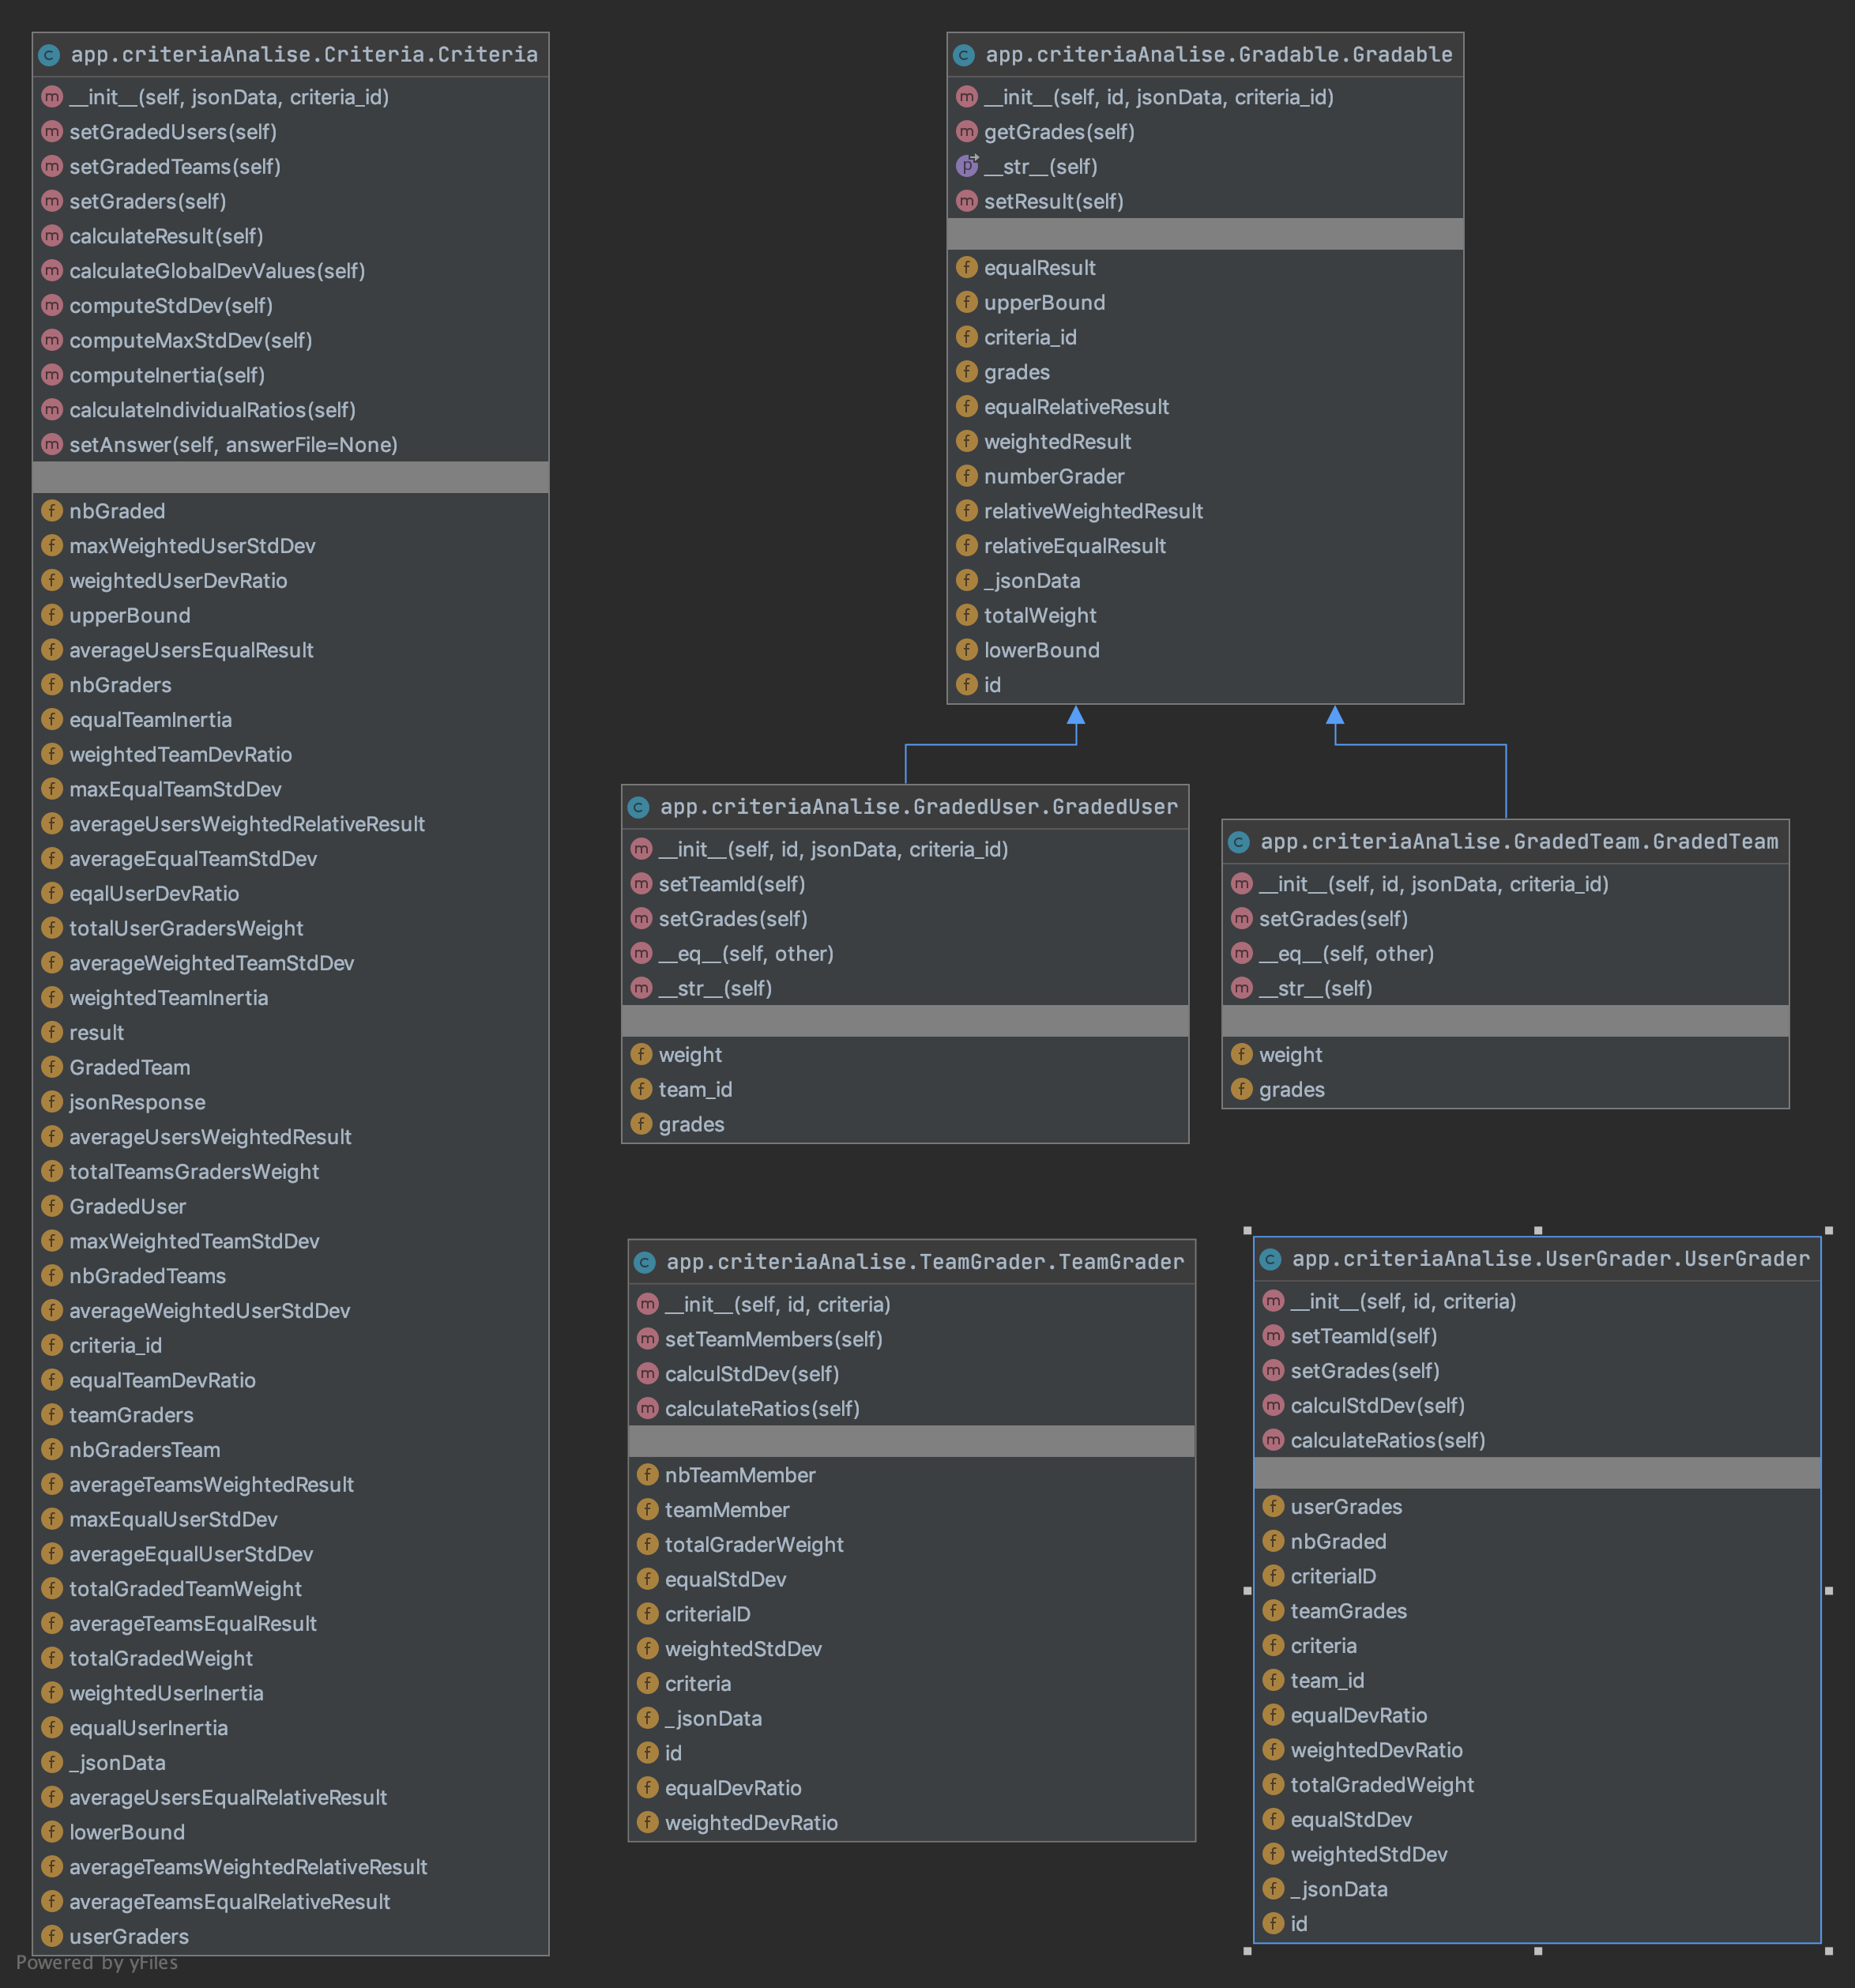
\includegraphics[width=15cm]{criteriaAnalise.png}
        \caption{Diagramme de classe de la partie calcul par critère}
    \end{figure}
    \newpage
    \subsection{Le module de calcul par phase ou activité}
        Cette partie a été finalement faite en fonctionnel et non pas en objet, car ce n'était pas nécessaire au vu de la simplicité de cette partie. 
    
\section{Remarques liées à l'utilisation par l'appli Serpico}
Il a été décidé de séparer complètement les résultats liés à l'évaluation de phase et de user. Ainsi, ce service est appelé deux fois dans le cas ou une phase évalue et la phase et les \usr. Dans le cas ou on appelle le framework quand la phase est évaluée, elle est considérée comme un \usr{} passif, avec un poids de 1, et un id de -1 (le poids n'importe peu, dans ce cas la phase est le seul utilisateur noté).
\section{Mise en prod et utilisation}
Le code est déployé sur le premier serveur de Serpico, voir le Readme pour plus de détails.
%docker build 
\end{document}